\documentclass[preprint,12pt]{elsarticle}
\usepackage{amsmath,amssymb,booktabs,graphicx}
\usepackage{xeCJK}
\usepackage{hyperref}
\hypersetup{hidelinks}
\journal{Journal of Computational Science}

\begin{document}
\begin{frontmatter}
\title{科学机器学习中可微科学计算基元的可靠性规范与跨后端验证}
\author[mech]{胡宁\corref{cor1}}
\ead{huning@hdu.edu.cn}
\author[cs]{段海涛}
\ead{25050509@hdu.edu.cn}
\author[math]{李书群}
\ead{Shuqun.Li24@student.xjtlu.edu.cn}
\author[ucsc]{胡初扬}
\ead{chu207@ucsc.edu}
\address[mech]{School of Mechanical Engineering, Hangzhou Dianzi University, Hangzhou, China}
\address[cs]{School of Computer Science, Hangzhou Dianzi University, Hangzhou, China}
\address[math]{School of Mathematics and Physics, Xi'an Jiaotong--Liverpool University, Suzhou, China}
\address[ucsc]{Department of Computer Science and Engineering, University of California, Santa Cruz, CA 95064, USA}
\cortext[cor1]{通讯作者。ORCID：胡宁 0000-0002-2718-0385；段海涛 0009-0006-4611-8639；李书群 0009-0007-1787-685X；胡初扬 0009-0007-9255-018X。}

\begin{abstract}
科学机器学习日益将传播子、矩阵函数作用、积分步和结构化残差块作为可组合的可微科学计算基元。然而，数值函数值精度、参数梯度、参数标定和模块复用通常没有在同一份可复现契约下评估。本文提出一种与具体后端无关的可靠性规范，针对批量可微映射 $y=P(x;\theta)$，要求明确适用域、参考求值器、函数值与梯度检查、参数标定、模块复用、分布外与长时域测试以及设备感知性能记录。我们以 Mittag--Leffler 谱层、矩阵指数作用、定步长线性 RK4 步进和 Logistic 方程 RK4 步进作为四类后端进行实例化验证。结果按后端分别报告，不合并为一个跨数学域的精度排名。矩阵指数和两类 RK4 后端在声明的低维域上通过函数值、梯度、标定、模块复用、分布外和长时域检查。共同神经 OOD 任务显示，基元组合可以改善 Logistic 后端，但并不普遍改善矩阵后端；这一负结果正是规范的组成部分，因为它将可微性可靠与任务预测收益区分开来。当前实现提供注册表和可审计 JSON 报告，但其边界仍是受控基准域，而不是通用求解器库。
\end{abstract}
\begin{keyword}
科学机器学习 \sep 可微基元 \sep 自动微分 \sep 数值可靠性 \sep 参数标定 \sep 可复现性
\end{keyword}
\end{frontmatter}

\paragraph{关键词：} 科学机器学习；可微基元；自动微分；数值可靠性；参数标定；可复现性

\section{引言}
科学机器学习模型正在将学习模块与传播子、矩阵函数作用、积分步和结构化残差块等数值映射组合起来。一个基元在软件层面“可微”，并不意味着它具有足够的函数值精度、稳定的参数敏感性或可靠的参数标定能力；反之，前向计算准确也不能单独证明其适合优化和重复组合。

本文研究的是缺失的评估契约，而不是新的通用求解器。我们定义一种可移植规范，明确回答四个问题：函数值在声明域内是否准确，参数梯度是否可信，参数能否从观测中标定，以及基元能否嵌入神经模块和物理目标中复用。分布外、长时域、批量与设备以及有限梯度检查作为附加可靠性门槛。

本文贡献包括：一套与后端无关的基元契约和标准化审计模式；一个包含注册表、性能记录和审计接口的 Python 实现；覆盖分数阶传播子案例与三个非分数阶控制后端的证据；以及一个同时保留正面和负面结果的共同神经 OOD 任务。本文贡献是方法规范和可复现性导向的，不声称某一后端能够支配所有其他后端。

\section{相关工作与定位}
本文与 DiffTaichi 等可微物理编程系统\citep{hu2020difftaichi}、通用微分方程科学机器学习\citep{rackauckas2020universal}以及神经算子\citep{kovachki2023neuraloperator}互补。分数阶传播部分与离散分数阶微积分\citep{lubich1986discretized}、Mittag--Leffler 函数数值评估\citep{garrappa2015mittag,gorenflo2014mittag}和分数阶 Laplacian 综述\citep{lischke2020fractional}相联系。
本文与可微编程、神经算子、物理信息学习、矩阵函数方法和分数阶数值方法互补。上述方向提供算法和模型类别，本文则规定一个数值组件在被视为可复用 SciML 基元之前应具备哪些证据。本双语初稿暂不填入未经逐条核验的参考文献，正式投稿前再完成文献审查和引用映射。

\section{基元契约}
每个后端都公开批量映射
\begin{equation}
 y=P(x;\theta),
\end{equation}
并明确输入域、参数域、输出形状、数据类型策略、设备策略和参考求值器。该规范不要求所有基元具有相同数学结构，而要求每个结论都保留其有效域。

\subsection{可靠性维度}
函数值可靠性通过声明的参考结果测量绝对误差、相对误差和有限值率。可微性通过有限梯度率和方向导数误差评估。参数标定使用带噪观测，报告参数误差、收敛行为、随机种子变化，并在可行时与匹配的非梯度基线比较。模块复用至少包含神经模块和批量算子或物理目标两类组合。OOD、长时域以及批量/设备测试用于暴露边界行为，而不是把它们压缩为一个总分。

\section{软件实现}
\begin{figure}[t]
\centering
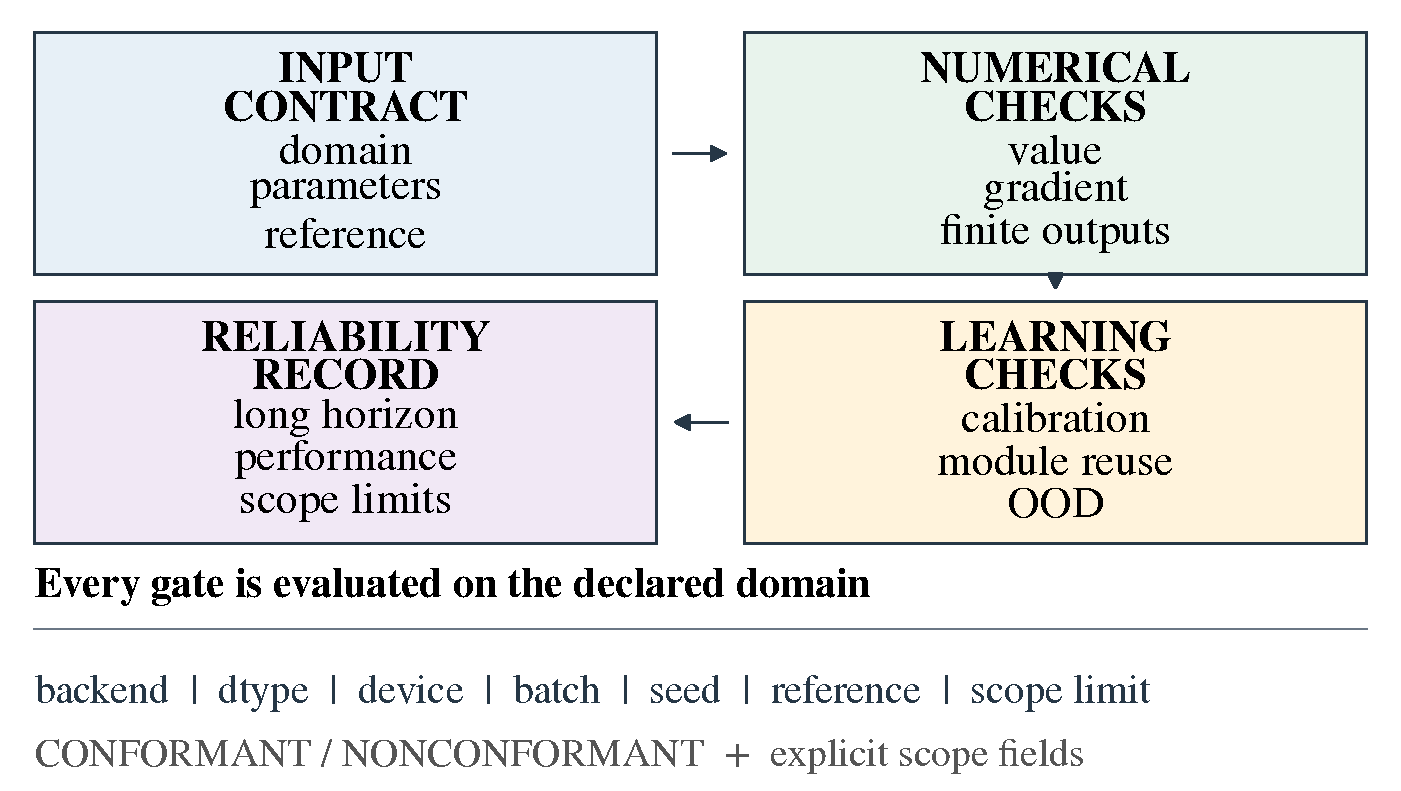
\includegraphics[width=0.98\linewidth]{figures/fig_protocol.pdf}
\caption{可微科学计算基元的可靠性工作流。每个门槛均在声明域内评估，并记录实现元数据和适用范围。}
\label{fig:protocol-zh}
\end{figure}
实现位于 \texttt{P4/dfsc\_protocol}。\texttt{audit\_value\_and\_gradient} 检查有限函数值和梯度；\texttt{audit\_batch\_and\_device} 检查批量运行与设备一致性；注册表记录各维度门槛状态和适用范围；性能模式记录延迟、吞吐、显存、数据类型和设备。JSON 报告由实验结果生成，论文表格不依赖手工抄录。

\section{实验设计}
当前验证采用低维受控问题，以保证参考值和方向导数可审计。四个后端为 Mittag--Leffler 谱层、矩阵指数作用、定步长线性 RK4 和 Logistic RK4。非分数阶后端用于检验规范能否跨越不同数值结构。除特别说明外，多随机种子实验使用 5 个种子。共同神经 OOD 任务使用 3 个种子、512 个训练任务、256 个测试任务、两个目标时刻（1.0 和 1.5）以及两种观测噪声（0.003 和 0.01），运行于 RTX 5070 Laptop GPU。

\section{实验结果}
\subsection{跨基元门槛覆盖}
注册表包含 4 个后端和 6 个要求维度：函数值、梯度、标定、模块复用、OOD 和长时域。我们进一步通过 P1 的公共工厂接口，以稳定混合配置重新运行了 MLSL。在声明的一维 Dirichlet、实负谱参数域内，相对于 80 位高精度参考级数的最大相对函数值误差为 $1.32\times10^{-12}$；alpha 和 beta 相对于中心差分的梯度误差分别为 $2.22\times10^{-9}$ 和 $5.00\times10^{-10}$。从 $(0.90,2.10)$ 初值出发，联合标定恢复为 $(\alpha,\beta)=(0.78003,1.80007)$。因此，MLSL 在六个协议门槛上均通过，但仍保留声明的适用范围限制。四个记录的状态均为“在范围限制下通过”。

\begin{table}[t]
\centering
\caption{代表性多种子可靠性结果。各后端指标分别报告，不合并为精度排名。}
\resizebox{\linewidth}{!}{%
\begin{tabular}{lccc}
\toprule
后端 & OOD 函数值误差 & 方向梯度误差 & 标定 L1 误差\\
\midrule
矩阵指数作用 & 长时域最大值 $4.27\times10^{-15}$ & $3.79\times10^{-11}$ & $3.11\times10^{-4}$\\
线性 RK4 步进 & OOD 最大值均值 $1.67\times10^{-3}$ & $2.48\times10^{-10}$ & $6.71\times10^{-4}$\\
Logistic RK4 步进 & OOD 最大值均值 $7.52\times10^{-6}$ & $4.41\times10^{-11}$ & $2.60\times10^{-2}\pm2.46\times10^{-2}$\\
\bottomrule
\end{tabular}%
}
\end{table}

矩阵指数作用在 5 个种子和 $0.02$ 至 $12$ 的时间范围内，长时域最大绝对误差均值为 $4.27\times10^{-15}$。线性 RK4 在步长 $0.41$--$0.80$ 的 OOD 测试中最大绝对误差均值为 $1.67\times10^{-3}$；在 $t=5$ 时，步长 0.05 和 0.20 的长时域误差分别为 $1.48\times10^{-9}$ 和 $4.23\times10^{-7}$。Logistic RK4 的 OOD 最大绝对误差均值为 $7.52\times10^{-6}$，但标定误差明显更大。这说明可靠性规范必须保留后端特定的误差预算。

\subsection{公开数据迁移验证}
我们进一步在两个具有来源记录的公开数据集上评估结构化基元。对于 GeoTES 中试规模热电偶数据（Zenodo DOI \href{https://doi.org/10.5281/zenodo.18979098}{10.5281/zenodo.18979098}），使用首个实测充放热周期进行标定，并在第二周期进行迁移测试。三个随机种子下，DFSC 加残差模型的第二周期相对误差为 $0.3619\pm0.0085$，纯 MLP 为 $0.3632\pm0.0071$，参数量分别为 750 和 1251。对于加热蒸汽注入温度剖面（Zenodo DOI \href{https://doi.org/10.5281/zenodo.15064388}{10.5281/zenodo.15064388}），留出工况 RMSE 分别为：直接 DFSC $43.33\pm0.56$ K，混合模型 $16.03\pm0.14$ K，纯 MLP $13.25\pm1.45$ K。后一结果作为负向任务级证据保留：可靠的可微基元并不意味着在所有数据集上都具有无条件的预测优势。这些实验支持真实数据迁移和适用范围诊断，而不支持通用物理辨识或普遍优越性论断。

为区分观测密度与外推时域的影响，我们进一步在首个完整周期内进行均匀抽样，并固定第二周期作为留出集。
在保留 40\% 观测时，混合模型的误差为 $0.3607\pm0.0082$，纯 MLP 为 $0.3657\pm0.0084$，参数量仍分别为
750 和 1251。在 20\%、60\% 和 100\% 观测比例下，混合模型未优于纯 MLP。因此，该结果应解释为中等数据预算下的条件性收益，而不是随观测量单调增强的 few-shot 优势。

\subsection{模块级 OOD 证据}
在共同神经任务中，Logistic 基元在两个目标时刻和两种噪声下均改善 OOD RMSE。例如在 $t=1.5$、噪声 0.003 时，基元模型为 $0.2340\pm0.0323$，纯 MLP 为 $0.2713\pm0.0096$。矩阵基元没有改善该任务：同一设置下分别为 $0.1998\pm0.0272$ 和 $0.1638\pm0.0097$。当前实现中基元模型训练也更慢。因此这里得到的是任务条件下的收益，而不是普遍预测优势。

\subsection{批量与 GPU 性能}
在 RTX 5070 Laptop GPU 上，三个通用后端在 batch 为 1、64、256 和 1024、float64 条件下均产生有限输出。吞吐随 batch 增大而提升，但这些结果是实现级性能记录，不构成跨数学域速度排名。性能记录同时保存预热次数、同步计时、峰值显存、数据类型和输出形状，以便未来后端按同一格式比较。

\section{讨论与适用边界}
\begin{figure}[t]
\centering
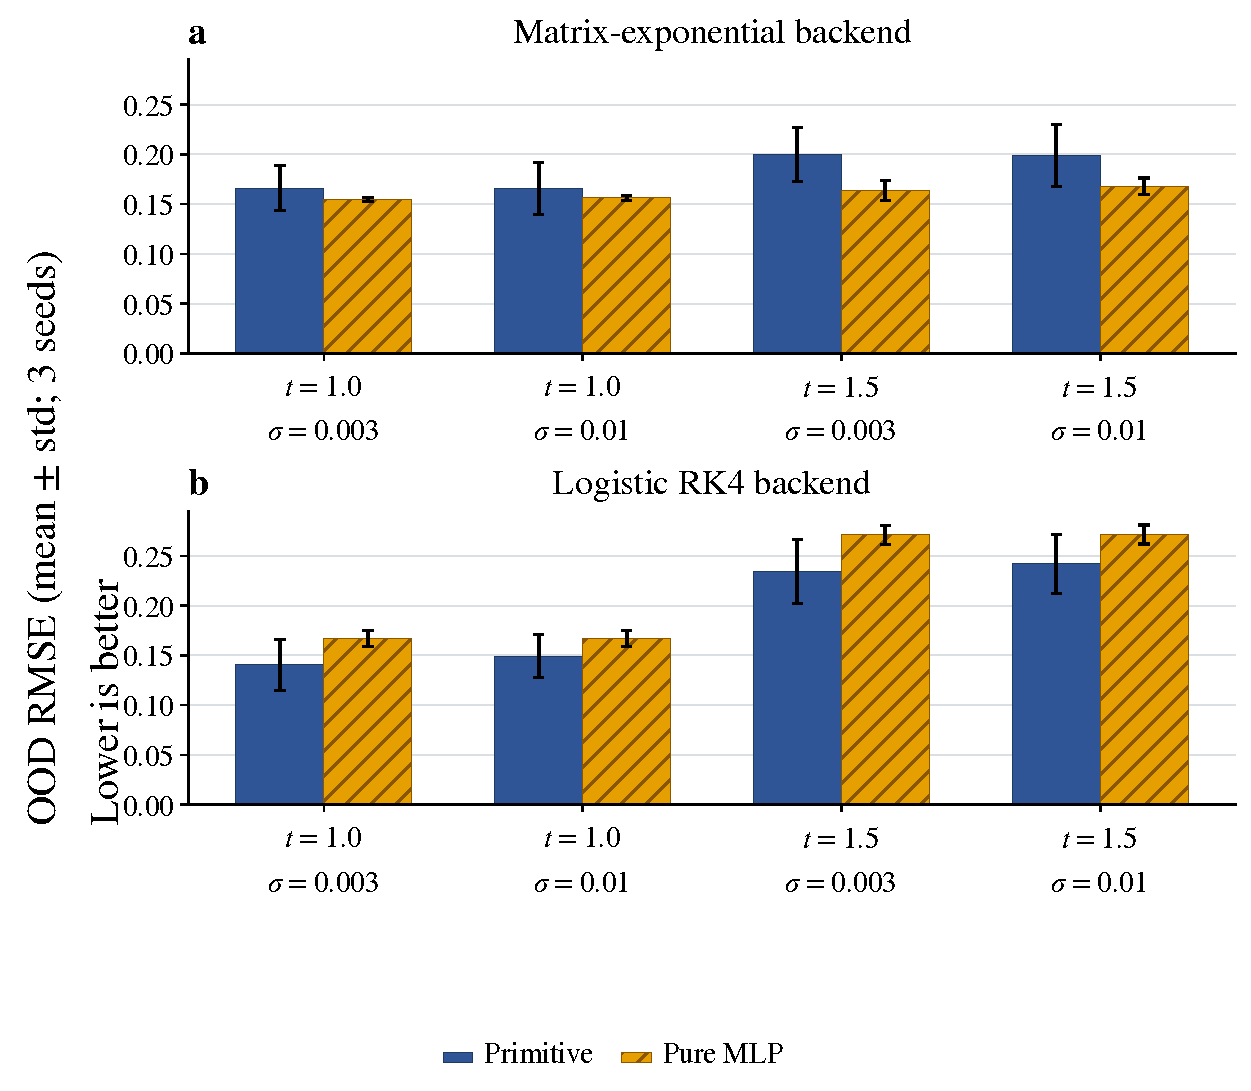
\includegraphics[width=0.98\linewidth]{figures/fig_common_ood.pdf}
\caption{共同模块级 OOD 任务。Logistic 基元在测试设置下改善 OOD RMSE，而矩阵基元并未普遍优于纯 MLP 控制。具体均值和标准差见源 JSON。}
\label{fig:common-ood-zh}
\end{figure}
当前证据支持规范的跨后端复用，不支持通用求解器优越性。研究结合了低维受控域、两个公开数据迁移测试和 PyTorch 执行路径，尚未验证变阶或分布阶分数阶算子、复杂几何、非结构网格、JAX/Julia 后端或通用物理辨识。在这些工作完成前，不能把本文描述为完整分数阶求解器库。

\section{可复现性与软件可用性}
实验脚本、JSON 结果、注册表/性能模式、软件测试和论文数据构建脚本均位于公开仓库 \href{https://github.com/hzhooning-art/DFSC}{github.com/hzhooning-art/DFSC} 的 P4 目录。论文表格可通过 \texttt{python paper/build\_paper\_data.py} 重新生成。托管 CPU 工作流已在 GitHub Actions 中通过，对应的软件提交为 \texttt{20fab75}，运行记录为 \href{https://github.com/hzhooning-art/DFSC/actions/runs/31581391771}{31581391771}；当前本地测试也已通过。仓库保存了实现和审计结果，独立外部复现仍作为推荐的进一步检查，不将其表述为已经完成的结果。

\section{结论}
\begin{figure}[t]
\centering
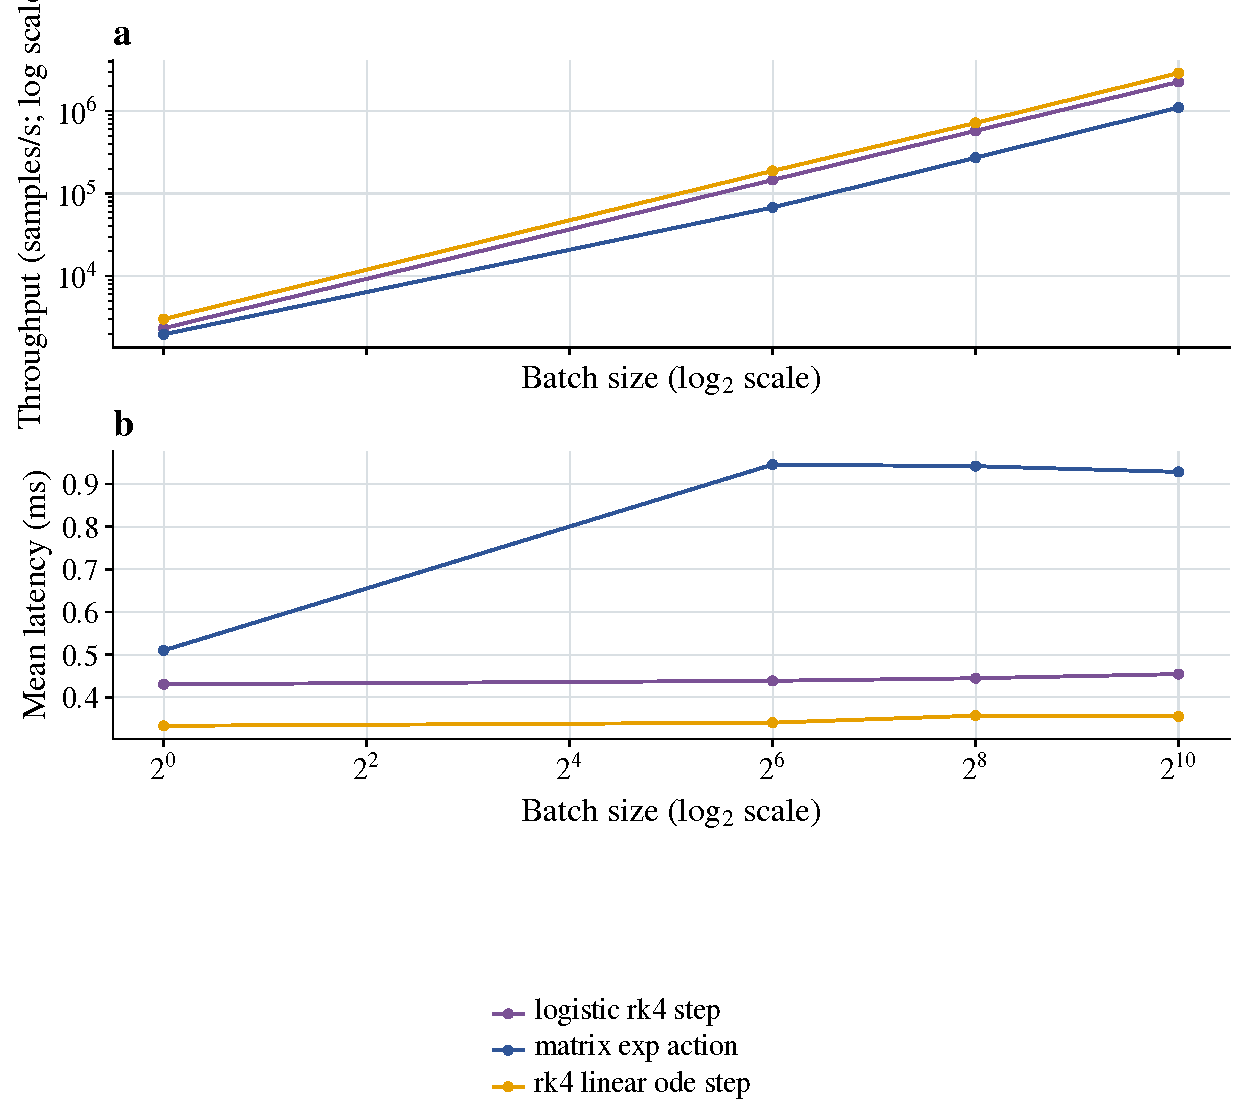
\includegraphics[width=0.86\linewidth]{figures/fig_gpu_profile.pdf}
\caption{RTX 5070 Laptop GPU 上的 batch 吞吐画像。曲线仅表示声明低维后端的实现级性能，不构成跨数学域速度排名。}
\label{fig:gpu-profile-zh}
\end{figure}
本文提出并验证了面向 SciML 可微科学计算基元的可靠性规范。通过分别检查函数值、梯度、参数标定、模块复用、OOD、长时域和硬件性能，该规范使论断可审计，并保留负面结果。当前证据支持在声明域内复用这一评估和软件接口，MLSL 作为分数阶案例提供动机。更广数值域和独立外部验证仍是形成更强生态论断的必要条件。

\section*{数据与代码可用性}
代码和生成的 JSON 报告位于 P4 项目目录。只有在完成对应软件 release 并核验后，才应在正式稿件中填写公开 release 和 DOI。

\section*{CRediT 作者贡献声明}
胡宁：概念化、方法学、软件、验证、形式化分析、调查、数据整理、可视化、初稿撰写、审阅与编辑。段海涛：方法学、软件、验证、调查、审阅与编辑。李书群：验证、调查、审阅与编辑。胡初扬：验证、调查、审阅与编辑。

\section*{利益冲突声明}
作者声明不存在可能影响本文研究工作的已知经济利益冲突或个人关系。

\section*{生成式人工智能与人工智能辅助技术声明}
最终声明应根据目标期刊政策，并在全体作者审核最终稿后填写。

本文准备过程中使用了人工智能辅助工具进行语言编辑、稿件结构整理、双语内容一致性检查以及代码和文档审阅。全体作者已对相关文本、数值论断、参考文献和软件陈述进行审核、修改与核验，并对最终内容承担全部责任。人工智能工具未用于生成或伪造实验数据。

\bibliographystyle{elsarticle-num}
\bibliography{references}

\end{document}
